\section{Приложение} \label{Приложение}

\subsection{Приложение 1} \label{Приложение 1}
Схема экспериментальной установки приведена на рис. 1
\begin{figure}[ht]
    \center{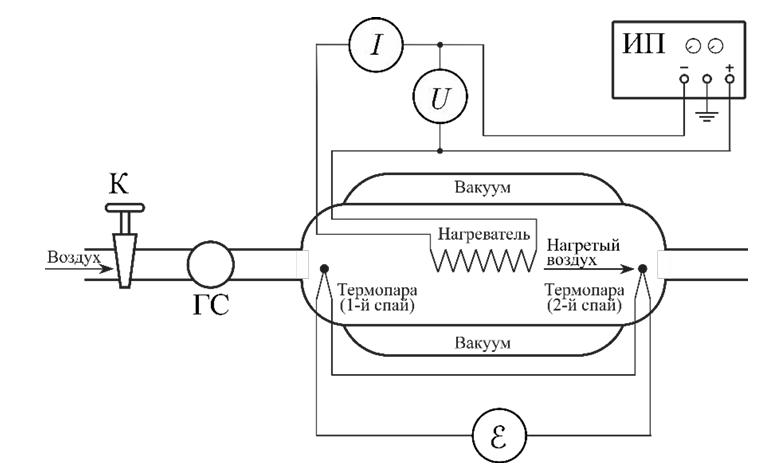
\includegraphics[scale=0.7]{img/exp_ustanovka_2.png}}
    \begin{center}       
        Рис. 1. Экспериментальная установка
    \end{center}
\end{figure}

Установка состоит из калориметра, через который прокачивается воздух, нагнетаемый компрессором. На пути воздуха перед калориметром расположен газовый счетчик (ГС) и кран (К) для регулировки расхода воздуха. Калориметр представляет собой стеклянную трубку с двойными стенками, запаянную с торцов. На внутреннюю поверхность стенок трубки нанесено серебряное покрытие для минимизации потерь энергии за счет излучения. Воздух из пространства между стенками откачан до высокого вакуума ($10^{-5}$ торр) для минимизации потерь энергии за счет теплопроводности. 

В калориметр встроен нагревательный элемент, представляющий собой нихромовую проволоку, намотанную на пенопласт. Нагреватель расположен в потоке воздуха, прокачиваемого через калориметр. Нагрев проволоки производится с помощью источника постоянного тока (ИП).

\subsection{Предложение 2} \label{Приложение 2}

Считая воздух смесью двухатомных идеальных газов, теоретическое значение теплоемкости $C_p$ при постоянном давлении определяется выражением:
\begin{equation}
    C_p = 3.5\nu R
\end{equation}
$\nu$ - количество молей воздуха

Количество теплоты, которое необходимо передать воздуху для нагрева его на $\Delta T = \SI{1}{\celsius}$ равно
\begin{equation}
    Q = C_p \Delta T = C_p = 3.5\nu R \label{eq: Q}
\end{equation}
Мощность нагревателя $N$ выражается через $Q$ как
\begin{equation}
    N = \frac{\delta Q}{dt} \label{eq: N}
\end{equation}
Подставляя \eqref{eq: Q} в \eqref{eq: N}, получаем
\begin{equation}
    N = 3.5R\frac{d\nu}{dt} \label{eq: N_2}
\end{equation}
Выразим производную $\frac{d\nu}{dt}$ через уравнение Менделеева-Клапейрона:
\begin{equation}
    PV = \nu RT \Rightarrow \nu = \frac{PV}{RT} \Rightarrow \frac{d\nu}{dt} = \frac{P}{RT} \cdot \frac{dV}{dt} \label{eq: proizv}
\end{equation}
Подставляя \eqref{eq: proizv} в \eqref{eq: N_2}, получаем
\begin{equation}
    N = 3.5 \frac{P}{T} \frac{dV}{dt} \label{eq: N_3}
\end{equation}
Так как $N = I_0^2 R_\text{н}$, где $R_\text{н}$ - сопротивление нагревателя, то, приравнивая данное выражение к \eqref{eq: N_3}, получаем
\begin{equation}
    I_0^2 R_\text{н} = 3.5 \frac{P}{T} \frac{dV}{dt} \Rightarrow I_0 = \sqrt{3.5 \frac{P}{TR_\text{н}} \frac{dV}{dt}} \label{eq: I_0}
\end{equation}

\subsection{Приложение 3} \label{Приложение 3}
\begin{table}[h]
    \centering
    \begin{tabular}{|c|c|c|c|c|c|c|c|}
    \hline
    $I, \text{мА}$ &  $U, \text{В}$ & $N, \text{Вт}$ & $R_{\text{н}}, \text{Ом}$ & $E, \text{мВ}$ & $\Delta T, \celsius$ & $\sigma_{\Delta T}, \celsius$ & $\sigma_N, \text{мВт}$ \\ \hline
    77.23  & 2.77 & 0.20  & 37  & 0.037  & 0.91 & 0.025 & 0.72 \\ \hline
    111.97 & 4.00 & 0.45  & 37  & 0.078  & 1.92 & 0.025 & 1.12 \\ \hline
    140.58 & 5.03 & 0.71  & 37  & 0.127  & 3.12 & 0.025 & 1.41 \\ \hline
    188.30 & 6.74 & 1.27  & 37  & 0.226  & 5.55 & 0.025 & 1.88 \\ \hline
    223.40 & 7.79 & 1.74  & 37  & 0.320  & 7.86 & 0.025 & 2.23 \\ \hline
    172.56 & 6.17 & 1.06  & 37  & 0.186  & 4.57 & 0.025 & 1.73 \\ \hline
\end{tabular}
    \caption{Зависимость $N(\Delta T)$ при $q = 0.2\frac{\text{г}}{\text{с}}$, N - мощность нагревателя, $\Delta T$ - разность температур воздуха, $q$ - расход воздуха}
    \label{tab:q1}
\end{table}
(описание всех переменных в таблице)

\begin{table}[h]
    \centering
    \begin{tabular}{|c|c|c|c|c|c|c|c|}
    \hline
    $I, \text{мА}$ &  $U, \text{В}$ & $N, \text{Вт}$ & $R_{\text{н}}, \text{Ом}$ & $E, \text{мВ}$ & $\Delta T, \celsius$ & $\sigma_{\Delta T}, \celsius$ & $\sigma_N, \text{мВт}$ \\ \hline
    45.47  & 1.63 & 0.08  & 37  & 0.035  & 0.86 & 0.025 & 0.45 \\ \hline
    68.57  & 2.46 & 0.17  & 37  & 0.083  & 2.04 & 0.025 & 0.69 \\ \hline
    112.22 & 4.01 & 0.45  & 37  & 0.220  & 5.41 & 0.025 & 1.12 \\ \hline
    133.32 & 4.77 & 0.64  & 37  & 0.315  & 7.74 & 0.025 & 1.33 \\ \hline
    139.32 & 4.98 & 0.69  & 37  & 0.345  & 8.48 & 0.025 & 1.39 \\ \hline
\end{tabular}
    \caption{Зависимость $N(\Delta T)$ при $q = 0.07\frac{\text{г}}{\text{с}}$, N - мощность нагревателя, $\Delta T$ - разность температур воздуха, $q$ - расход воздуха}
    \label{tab:q2}
\end{table}
\newpage

\subsection{Приложение 4} \label{Приложение 4}
\begin{table}[h]
    \centering
    \begin{tabular}{|c|c|c|c|}
    \hline
    $k, \frac{\text{Вт}}{\celsius}$ &  $q, \frac{\text{г}}{\text{с}}$ & $\sigma_q \cdot 10^{-7}, \frac{\text{г}}{\text{с}}$ & $\sigma_k \cdot 10^{-3}, \frac{\text{Вт}}{\celsius}$  \\ \hline
    0.22  & 0.20 & 4  & 4.0 \\ \hline
    0.08  & 0.07 & 4  & 0.7  \\ \hline
\end{tabular}
    \caption{Зависимость $k(q)$, $k$ - угловой коэффициент зависимости $N(\Delta T)$, $q$ - расход воздуха}
    \label{tab:q3}
\end{table}

\subsection{Приложение 5} \label{Приложение 5}
\begin{table}[h]
    \centering
    \begin{tabular}{|c|c|c|}
    \hline
    $\frac{N_{\text{пот}}}{N}$ &  $q, \frac{\text{г}}{\text{с}}$ & $\sigma_{\frac{N_{\text{пот}}}{N}}\cdot 10^{-3}$ \\ \hline
    0.086  & 0.20  & 15 \\ \hline
    0.238  & 0.07  & 6 \\ \hline
\end{tabular}
    \caption{Значения $\frac{N_{\text{пот}}}{N}$ при фиксированных расходах $q$ воздуха}
    \label{tab:q4}
\end{table}

\subsection{Приложение 6} \label{Приложение 6}
\begin{center}
    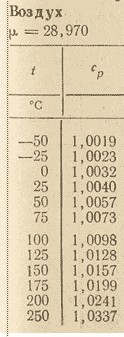
\includegraphics[width=0.3\textwidth]{img/ud_teplo.png}
    
    Таблица значений удельной теплоемкости воздуха при постоянном давлении при различных температурах.
\end{center}

\subsection{Формулы для расчета погрешностей}
\subsubsection{Расчет погрешности углового коэффициента графика $N(\Delta T)$}
\[\sigma_k = \frac{1}{\sqrt{n}}\sqrt{\frac{\langle N^2 \rangle - {\langle N \rangle}^2}{\langle \Delta T^2 \rangle - {\langle \Delta T \rangle}^2} - k^2}\] $n$ - количество экспериментальных точек.

\subsubsection{Расчет погрешности углового коэффициента и свободного члена графика $k(q)$}
\[\sigma_{c_p} = \frac{1}{\sqrt{n}}\sqrt{\frac{\langle k^2 \rangle - {\langle k \rangle}^2}{\langle q^2 \rangle - {\langle q \rangle}^2} - c_p^2}\]
\[\sigma_\alpha = \sigma_{c_p} \cdot \sqrt{\langle q^2 \rangle - {\langle q \rangle}^2}\]
\subsubsection{Расчет погрешности измерения мощности нагревателя}
\[N = U \cdot I\]
\[\epsilon_N = \epsilon_U + \epsilon_I = \frac{\sigma_U}{U} + \frac{\sigma_I}{I}\]
\[\frac{\sigma_N}{N} = \frac{\sigma_U}{U} + \frac{\sigma_I}{I}\]
\[\sigma_N = N(\frac{\sigma_U}{U} + \frac{\sigma_I}{I})\]
\subsubsection{Расчет погрешности вычисления доли тепловых потерь}
\[\frac{N_\text{пот}}{N} = \frac{\alpha}{k}\]
\[\epsilon_{\frac{N_\text{пот}}{N}} = \epsilon_\alpha + \epsilon_k = \frac{\sigma_\alpha}{\alpha} + \frac{\sigma_k}{k}\]
\[\frac{\sigma_{\frac{N_\text{пот}}{N}}}{\frac{N_\text{пот}}{N}} = \frac{\sigma_\alpha}{\alpha} + \frac{\sigma_k}{k}\]
\[\sigma_{\frac{N_\text{пот}}{N}} = \frac{N_\text{пот}}{N}(\frac{\sigma_\alpha}{\alpha} + \frac{\sigma_k}{k})\]